\section{Image Processing Methods}

All MRI volumes will be processed using Advanced Normalization Tools
(ANTs) \href{http://www.picsl.upenn.edu/ANTS}{(click here for
link)}\cite{Avants2011a,Avants2011,Murphy2011,Tustison2010,Tustison2011,Tustison2011a}
via previously reported procedures validated as highly accurate
\cite{Klein2009,Klein2010,Murphy2011,Avants2011}.  In general, ANTs-based
processing for multiple modalities is based on, first, defining a
template to guide the population normalization and segmentation
procedures \cite{Avants2011a,Avants2011}.  Traditionally, this
approach was used for single modalities but, more recently, is
exetended for multiple modalities via multiple-modality cohort-specific templates
that capture the average shape and appearance of T1, DTI and
functional images, as in \cite{Kim2010,Avants2011a,Jain2012,Tustison2012}.  We use the
template to guide brain extraction for all modalities and subsequent
tissue or neuroanatomical parcellation \cite{Avants2011a}.  
This general procedure allows several complementary measurements to be
extracted from neuroimaging including 
cortical thickness via DiReCT \cite{Das2009a}, mean diffusion which
may be sensitive to neuronal death \cite{}, fractional anisotropy,
cerebral blood flow from ASL \cite{Jain2012} or graph connectivity metrics from ASL or
BOLD \cite{}.  These measurements, taken together, yield a
multispectral picture of brain health or disease that may have
significant translational value for diagnostics \cite{McMillan2013a} and prognostics \cite{Yuh2013}.

Justification for each modality is described briefly: 

\noindent{\em Jacobian-based Volume from T1-weighted MRI:}  T1 MRI is
typically the highest resolution anatomical image routinely collected
in both clinical and research MRI protocols.  Image registration
methods are able to use T1 MRI to obtain voxel-wise measurement of the
subject structural volume relative to a group local template or
relative to a baseline timepoint.  These measurements are used in
Tensor-Based Morphometry (TBM) which, when performed symmetrically as
in my prior work \cite{Yushkevich2010a,Das2012}, is highly accurate
and provides detailed information on shape change over time
\cite{Brambati2007998,Hua2011,Kim2013} or across a population \cite{Kim2008,Massimo2009,Morgan2011,Hanson2010,Hanson2012}.

\noindent{\em Cortical thickness from T1-weighted MRI:}  A measurement that is both sensitive and specific in neurodegeneration \cite{Stricker2012,Libon2012,McMillan2013} and which is associated with cognitive decline \cite{Dickerson2011,Avants2010}.  

\noindent{\em Fractional anisotropy (FA) from DTI:}  A measurement of white matter integrity that may reveal the connectivity components of neurodegeneration \cite{Zhang2009B}, potentially captures a different aspect of the disease process \cite{Englund2004JN} and may differentiate tau and TDP-43 effects \cite{McMillan2013JNNP}.    

\noindent{\em BOLD Network Analysis:} BOLD-based network analysis
\cite{Spoormaker2010,Sanz-Arigita2010} has emerged as a powerful tool
with specific value in both brain injury
\cite{Mayer2011,Scheibel2012,Zhou2013}, the study of intervention
strategies \cite{Roy2010,FeldsteinEwing2011} and measurement of pain
\cite{Mayhew2013}.

\noindent{\em Cerebral blood flow (CBF) from ASL:}  This functional
quantitative measure (versus the relative values provided by BOLD) has
the potential to reveal alterations in the brain due to injury
\cite{Kim2008}, pain \cite{Howard2011}, pharmacological intervention \cite{Black2010,Jenkins2012} or that precede visible structural change and may
indicate cortical reorganization \cite{Hayward2010}.  ASL-based CBF
also accurately recapitulates PET imaging in Alzheimer's disease \cite{Chen2011,Mak2012}.
CBF is a more repeatable functional measurement than BOLD
\cite{Liu2007,Aguirre2012}, may be used in network analysis in lieu of
or combination with 
BOLD \cite{Duda2013} and provides a unique view on the brain complementary to DTI and T1.  

\subsection{ANTs volumetric-based cortical thickness estimation pipeline}

The ANTs-based cortical thickness estimation workflow is illustrated 
in Figure \ref{fig:pipeline}.  The steps are as follows:
\begin{enumerate}
  \item initial N4 bias correction on input anatomical MRI,
  \item brain extraction using a hybrid segmentation/template-based strategy,
  \item alternation between prior-based segmentation and white matter posterior
        probability weighted bias correction,
  \item DiReCT-based cortical thickness estimation, and
  \item optional normalization to specified template.
\end{enumerate}
Each component, including both software and data, is briefly detailed 
below with the relevant references for additional information. 


%We also note that each component is publicly available with all ANTs 
%algorithms available as open source.%
%\footnote{
%http://www.picsl.upenn.edu/ANTS
%}
Additionally, the coordination of all the algorithmic components is
encapsulated in the shell scripts \verb#antsCorticalThickness.sh# with
subcomponents delegated to \verb#antsBrainExtraction.sh# 
and \verb#antsAtroposN4.sh#.  This includes
optimal parameters for each of the algorithmic components which has worked
well for our processing and which are used to acquire the results 
described in this work.

%\lstset{frame = tb,
%        framerule = 0.25pt,
%        float,
%        fontadjust,
%        backgroundcolor={\color{listlightgray}},
%        basicstyle = {\ttfamily\scriptsize},
%        keywordstyle = {\ttfamily\color{listkeyword}\textbf},
%        identifierstyle = {\ttfamily},
%        commentstyle = {\ttfamily\color{listcomment}\textit},
%        stringstyle = {\ttfamily},
%        showstringspaces = false,
%        showtabs = false,
%        numbers = none,
%        numbersep = 6pt,
%        numberstyle={\ttfamily\color{listnumbers}},
%        tabsize = 2,
%        language=,
%        floatplacement=!h,
%        caption={\small \baselineskip 12pt DiReCT long command line menu which is invoked using the `{\ttfamily {-}{-}help}' option.  The short command line menu is obtained by typing `{\ttfamily {-}h}'}.,
%        captionpos=b,
%        label=listing:long
%        }
%\lstsetcpplong
%\begin{lstlisting}
%This script, apb.sh, performs T1 anatomical brain 
%processing where the following steps are currently 
%applied:
%
%  1. Brain extraction
%  2. Brain 3-tissue segmentation
%  3. Cortical thickness
%  4. (Optional) registration to a template
%
%Usage:
%
%abp.sh -d ImageDimension
%       -i T1Image.nii.gz
%       -e BrainExtractionTemplate
%       -m BrainExtractionProbabilityMask
%       -l BrainParcellationTemplate
%       -p BrainParcellationProbabilityMask
%       <OPTARGS>
%       -o OutputPrefix
%
%Example:
%
%abp.sh -d 3 
%       -i t1.nii.gz 
%       -e brainWithSkullTemplate.nii.gz 
%       -m brainPrior.nii.gz 
%       -l corticalLabels.nii.gz 
%       -p corticalLabelPriors.nii.gz 
%       -o output
%
%Compulsory arguments:
%
%     -d:  ImageDimension                        2 or 3 (for 2 or 3 dimensional single image)
%     -a:  Anatomical T1 image                   typically T1.
%     -e:  Brain extraction template             Anatomical template created using e.g. LPBA40 data set with
%                                                buildtemplateparallel.sh in ANTs.
%     -m:  Brain extraction probability mask     Brain probability mask created using e.g. LPBA40 data set which
%                                                have brain masks defined, and warped to anatomical template and
%                                                averaged resulting in a probability image.
%     -l   Brain segmentation template           Anatomical template for brain segmentation.  E.g. NIREP template
%                                                with labels.
%     -p   Brain segmentationpriors              Label probability priors corresponding to the image specified
%                                                with the -l option.  Specified using c-style formatting, e.g.
%                                                -p labelsPriors\%02d.nii.gz.
%     -o:  OutputPrefix                          The following images are created using the specified prefix:
%                                                  * /Users/ntustison/Data//tmp13243//tmpN4Corrected.nii.gz
%                                                  * /Users/ntustison/Data//tmp13243//tmpExtractedBrain.nii.gz
%                                                  * /Users/ntustison/Data//tmp13243//tmp3TissueBrainSegmentation.nii.gz
%                                                  * /Users/ntustison/Data//tmp13243//tmpCorticalThickness.nii.gz
%                                                  * /Users/ntustison/Data//tmp13243//tmpSurfaceCurvature.nii.gz
%
%Optional arguments:
%
%     -s:  image file suffix                     Any of the standard ITK IO formats e.g. nrrd, nii.gz (default), mhd
%     -t:  template for t1 registration
%     -k:  keep temporary files                  Keep brain extraction/segmentation warps, etc (default = false).
%     -w:  white matter label                    white matter label for segmentation (default = 3).
%     -g:  gray matter label                     cortical gray matter label for segmentation (default = 2)
%     -i:  max iterations for registration       ANTS registration max iterations (default = 50x100x20)
%\end{lstlisting}



\begin{figure*}
  \centering
  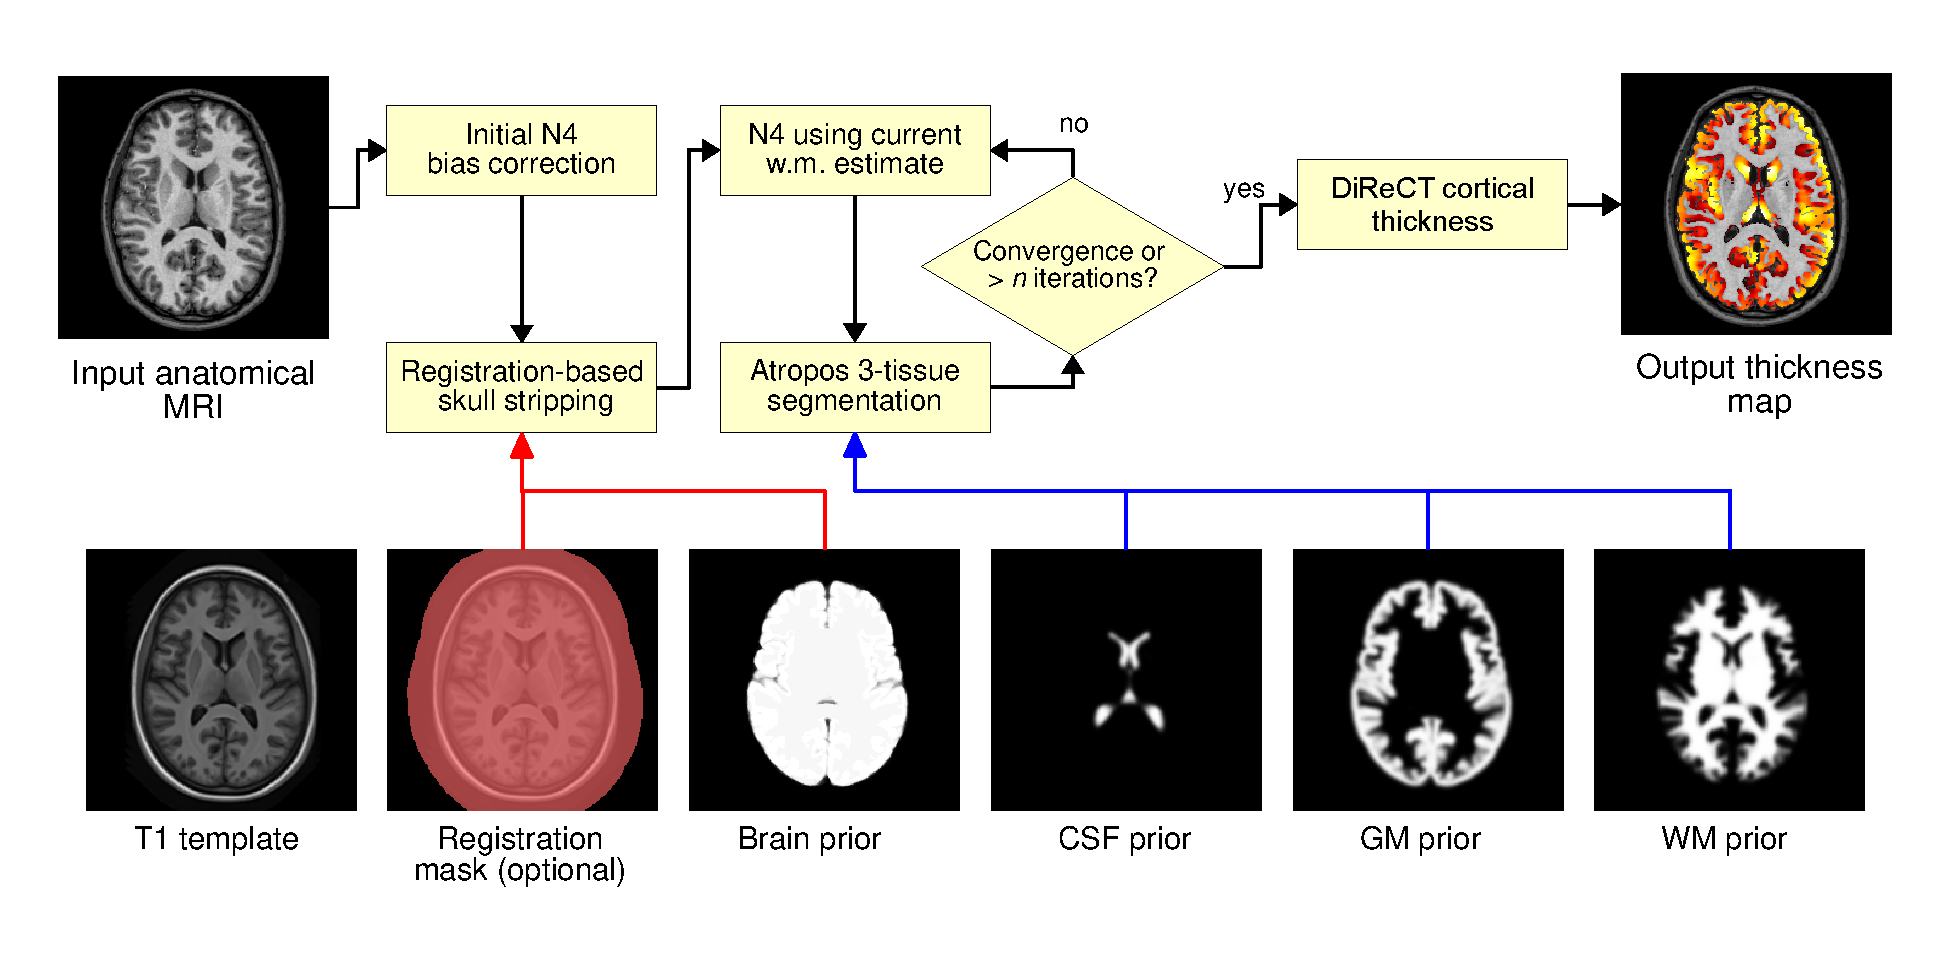
\includegraphics[width=170mm]{figs/Kapowski_pipeline2.pdf}
  \caption{Illustration of the main components of the ANTs processing 
  workflow containing all elements for determining cortical thickness. 
  Not shown is the optional subject to template registration.}
  \label{fig:pipeline}
\end{figure*}

\subsubsection{Anatomical template construction}

Normalizing images to a standard coordinate system
reduces intersubject variability in population studies.  Various
approaches exist for determining the normalized space such as the selection
of a pre-existing template based on a single subject, e.g. the Talairach
atlas \citep{Talairach1988}, or a publicly available averaged group of
subjects, e.g. the MNI \citep{Collins1994} or ICBM \citep{Mazziotta1995}
templates.  Additionally, mean templates constructed from labeled
data can be used to construct spatial priors for improving segmentation
algorithms.
The work of \cite{avants2010} explicitly models the geometric component of the 
normalized space during optimization to produce such mean templates.  Coupling the intrinsic symmetry of 
SyN pairwise registration \citep{Avants2011} and an
optimized shape-based sharpening/averaging of the template appearance, Symmetric Group
Normalization (SyGN) is a powerful framework for producing optimal population-specific
templates \citep{avants2010}.

%One challenge with standard templates is that they may inadvertently bias one's results by enabling better normalization of subjects to which the template is more similar.  This issue is exacerbated when dealing with populations that have high variance (e.g. due to disease) and/or when one's normalization method is low-dimensional (not flexible enough to capture large shape differences). 

%Population-specific templates alleviate some of
%the issues with other template approaches by deriving a most representative image from the population
%\citep{Good2001}.  Large deformation registration algorithms also reduce
%this confound by being less sensitive to the deformation distance
%between subject and target.  Some approaches combine both advantages,
%for instance, the diffeomorphic approach of Joshi et al. employs the
%SSD metric and a shape distance to bring the subject group of images
%into alignment \citep{Joshi2004}.  Variants
%include extension to multiple modalities \citep{Lorenzen2006} and small deformations
%\citep{Geng2009}.  These approaches iteratively minimize group difference in ``congealing''
%towards a representative image template \citep{Learned-Miller2006}.


The ANTs implementation of this technique is currently available as a shell script, 
\verb#buildtemplateparallel.sh# (a multivariate version is also available as
\verb#antsMultivariateTemplateConstruction.sh#).  Both scripts are distributed as part of
 the ANTs repository.
The latter script permits the construction of multimodal templates (e.g. 
T1-weighted, T2-weighted, proton density MRI and fractional anisotropy).  
Both scripts accommodate a variety of computational resources
for facilitating template construction.  These computational resource possibilities include:
\begin{itemize}
  \item serial processing on a single workstation, 
  \item parallelized processing on a single workstation with multiple cores using \verb#pexec#%
  \footnote{http://www.gnu.org/software/pexec/pexec.1.html},
  \item parallelized processing using Apple's XGrid technology%
  \footnote{https://developer.apple.com/hardwaredrivers/hpc/xgrid\_intro.html}, 
  \item parallelized processing using Sun Grid Engine for cluster-based systems%
  \footnote{http://www.oracle.com/technetwork/oem/grid-engine-166852.html}, and 
  \item parallelized processing using the Portable Batch System for cluster-based systems%
  \footnote{http://www.pbsworks.com/}.
\end{itemize}

For this work, database-specific templates were used during cortical thickness pipeline
processing for both brain extraction and brain segmentation steps.  Multivariate templates 
were constructed from the multimodal data sets.  However, their usage was based on the 
fact that they had been built previously for other work and not because they provide a 
discernible advantage over univariate templates (i.e. T1-only) for the proposed workflow.

%Given a set of representative images, 
%$\{I_1, I_2, \ldots, I_M\}$, optimization involves finding the set of paired
%diffeomorphic transformations, $\left\{\left(\phi^1_1, \phi^1_2\right), 
%\left(\phi^2_1, \phi^2_2\right), \ldots, \left(\phi^M_1, \phi^M_2\right) \right\}$,
%the optimal template appearance, $J^*$, and corresponding coordinate system, $\psi(\mathbf{x})$,
%which minimize the following cost function:
%\begin{align}
%  \sum_{m=1}^M \left[
%    D\left( \psi(\mathbf{x}), \phi^m_1(\mathbf{x}, 1) \right) + 
%    \Pi \left( I_m\left(\phi^m_2(\mathbf{x}, 0.5) \right), J^*\left(\phi^m_1(\mathbf{x}, 0.5) \right) \right)
%    \right]
%\end{align}
%where $D$ is the diffeomorphic shape distance, 
%\begin{align}
%  D\left(\phi(\mathbf{x}, 0), \phi(\mathbf{x}, 1)\right) = \int_{0}^1 \| v(\mathbf{x}, t) \|_L dt, 
%\end{align}
%dependent upon the choice of the linear operator, $L$, and
%$v$ is the diffeomorphism-generating velocity field, 
%\begin{align}
%  v\left(\phi(\mathbf{x}, t), t \right) = \frac{d\phi(\mathbf{x}, t)}{dt},\,\,\, \phi(\mathbf{x}, 0) = \mathbf{x}.
%\end{align}
%$\Pi$ is th
%e choice of similarity metric, often cross-correlation \citep{Avants2008a}, calculated in the 
%virtual domain midway between each individual image and the current estimate of the template. 
%
%With initial assignment of $\left\{\left(\phi^m_1, \phi^m_2\right)\right\}$ and $\psi(\mathbf{x})$ 
%to identity, iterative optimization
%involves estimating the pairwise transformations, estimation of the optimal template appearance, and 
%updating $\psi(\mathbf{x})$ by averaging the current estimate of $\left\{\phi_1^m\right\}$.  


\subsubsection{N4 Bias field correction}

Critical to quantitative processing of MRI is the minimization of
field inhomogeneity effects which causes artificial low frequency 
intensity variation across the image.  Large-scale studies, such
as the Alzheimer's Disease Neuroimaging Initiative (ADNI), employ
perhaps the most widely used bias correction algorithm, N3 \cite{sled1998}, 
as part of their standard protocol \citep{boyes2008}.

In \cite{tustison2010}, we introduced an improvement of N3, denoted as
``N4'', which demonstrates a significant increase in performance and convergence behavior
on a variety of data.  This improvement is a result of an enhanced 
fitting routine (which includes multi-resolution capabilities) and a modified optimization 
formulation.  For our workflow, the additional possibility of specifying
a weighted mask in N4 permits the use of a ``pure tissue'' probability map 
(described below)
calculated during the segmentation pipeline for further improvement of 
bias field estimation.  In addition to its public availability 
through ANTs and the Insight Toolkit, it has also been included in
the popular open source Slicer software package for visualization and medical
image computing \cite{fedorov2011}.

N4 is used in two places during the individual subject processing (cf. Figure
\ref{fig:pipeline}).  Following conversion of the raw dicom T1-weighted image
to Nifti format using our related \verb#Neuropipedream# set of raw image conversion
and organization tools%
\footnote{
http://sourceforge.net/projects/neuropipedream/
}, N4 is used to generate an initial bias corrected image for use in
brain extraction.  The input mask is created by adaptively thresholding 
the background from the foreground using Otsu's algorithm \cite{otsu1979}.
Following brain extraction, three-tissue segmentation involves iterating
between bias field correction using the current pure tissue 
probability map as a weight mask and then using that bias corrected image
as input to the Atropos segmentation step (described in the next section). 

\subsubsection{Atropos 3-tissue segmentation}

In \cite{Avants2011a} we presented an open source $n$-tissue segmentation software tool
(which we denote as ``Atropos'') attempting to distill 20+ years of active research in this area
particularly some of its most seminal work (e.g. \cite{zhang2001,ashburner2005}). 
Specification of prior probabilities includes spatially varying Markov Random Field modeling, 
prior label maps, and prior probability maps typically derived from our template building 
process.  Additional
capabilities include handling of multivariate data, 
partial volume modeling \cite{shattuck2001}, a memory-minimization mode,
label propagation, a plug-n-play architecture for incorporation of novel likelihood models
which includes both parametric and non-parametric models for both scalar and tensorial
images, and alternative posterior formulations for different segmentation tasks.

Due to the important interplay between segmentation and bias correction,
we perform multiple N4 $\Leftrightarrow$ Atropos iterations.
In order to better integrate Atropos and N4, we use  
a pure tissue probability weight mask generated from the 
posterior probabilities generated from the segmentation 
process.  Given $N$ labels and the corresponding $N$
posterior probability maps $\{ P_1, \ldots, P_N\}$ produced
during the segmentation process, the N4 weight mask is 
created at each N4 $\Leftrightarrow$ Atropos iteration from
\begin{align}
  P_{pure\,\,tissue}(\mathbf{x}) = \sum_{i=1}^N P_i(\mathbf{x}) \prod_{j=1, j \neq i}^N \left( 1 - P_j(\mathbf{x}) \right).
\end{align}
One of the key insights of the original N3 algorithm is the
observation that inhomogeneities cause the intensity values of
pure tissue peaks to spread in the intensity histogram as though
convolved with a Gaussian.  A core contribution of N3 is the
proposed corrective of deconvolving the intensity histogram to 
accentuate the tissue peaks coupled with a spatial smoothing 
constraint. The pure tissue probability mask
weights more heavily the voxels corresponding to pure tissue 
types (as determined by the segmentation) during the deconvolution process 
while minimizing the contribution of regions such as the gray/white matter 
interface where peak membership is ambiguous. 

\subsubsection{Brain extraction}

Brain extraction using ANTs combines template building, high-performance
brain image registration \citep{Avants2011}, and Atropos with topological refinements.  
An optimal template for brain extraction is 
generated offline using labeled brain data.  For example, in this work we use the LPBA40 data 
for generating a brain extraction template and a corresponding brain probability mask which is
available on the website associated with this submission. 

  The warped template probability map is thresholded at 0.5 and the resulting mask is dilated
with a radius of 2.  Atropos is used to generate an initial 3-tissue segmentation estimate within the mask
region.  Each of the three tissue masks undergo specific morphological operations which are then
combined to create a brain extraction mask for use in the rest of the
cortical thickness workflow.  \textcolor{blue}{does there need to be a
  bit more technical detail here?  while you can refer to the script,
  why perform these operations?  there are numerous references, most
  germane probably some recent stuff from J Prince ( i think ) and the
  freesurfer watershed approach which came from ... i forget ... maybe
  one of the french groups.}

A comparison using open access brain data with publicly available
brain extraction algorithms including AFNI's \verb#3dIntracranial#
\citep{ward1999}, FSL's \verb#BET2# \citep{smith2002}, Freesurfer's
\verb#mri_watershed# \citep{segonne2004}, and BrainSuite
\citep{dogdas2005} demonstrated that our combined
registration/segmentation approach \citep{avants2010a} performs at the
top level alongside BrainSuite (tuned) and FreeSurfer.
\textcolor{blue}{ok you have the segonne ref here ... }


\subsubsection{DiReCT (aka KellySlater/KellyKapowski) Cortical Thickness Estimation}

DiReCT was introduced 
in \cite{das2009} and made available in ANTs with the program \verb#KellySlater#.
Since then several improvements have been made and incorporated into the program
\verb#KellyKapowski#.%
\footnote{
Traditional academic discourse encountered in the published literature
rarely contextualizes peculiarities such as algorithmic nomenclature.
We briefly mention that
this was the source of a rare disagreement between the first two authors
based, as many disagreements are, on a simple misunderstanding and not an
affronting existential statement concerning a certain favorite sitcom
of the author's youth. 
}
Among the most significant advancements is that the more recent
implementation is multi-threaded, written in rigorous ITK coding style, and 
has been made publicly available through  ANTs complete with a unique user 
interface design developed specifically for ANTs tools.  


\subsubsection{DTI Processing with ANTs} 

%Phil --- see
%\href{www.ncbi.nlm.nih.gov/pubmed/23151955‎}{www.ncbi.nlm.nih.gov/pubmed/23151955}
% for content.
The first unweighted image in the diffusion sequence is used as the reference image for motion and distortion correction. The remaining unweighted images are rigidly aligned to the reference image and averaged; this average image is used as the reference image for affine correction of the diffusion-weighted images (DWI) for motion and distortion caused by the diffusion weighting gradients. A brain mask is computed by aligning the average DWI to a template, and warping the template brain mask into the subject space. Processing then continues on the brain-extracted image. Diffusion tensors are calculated using Camino \cite{Cook2006ISMRM} using an iterative weighted linear least squares algorithm \cite{Salvador2005HBM}.

Each T1-weighted image is segmented into gray matter, white matter and CSF using N4 bias correction \cite{tustison2010} and Atropos segmentation \cite{Avants2011a}. The white matter is used as a registration mask for alignment with the corresponding average DWI image. The DWI image is registered to the T1-weighted image using a transform composition derived by optimizing an initial rigid transformation followed by an optimized deformable (symmetric diffeomorphic using SyN \cite{Avants2011}) transform. The rigid transform is found by optimizing the alignment between the average DWI and the masked white matter T1-weighted image of the same subject, to account for motion. The resulting rigid transform is used to initialize distortion correction using the deformable transform.

The transformed DTI are warped to the template space by combining the intra-subject DWI to T1 warp with the warp previously defined to normalize the subject's T1 image to the template space. The correct anatomical orientation of the diffusion tensors is preserved by applying the preservation of principal direction method \cite{Alexander2001ITMI}, and scalar statistics such as FA and mean diffusivity are computed from the normalized diffusion tensors.


\subsubsection{Functional Image Processing}

We used AFNI (Cox, 1996) to motion-correct and spatially normalize the functional images, and to skull-strip and spatially normalize the anatomical images. Functional and anatomical images were normalized to the Colin brain template in Talairach space at 2 × 2 × 2-mm resolution. The FMRIB Automated Segmentation Tool (FAST; Zhang et al., 2001) was used to segment the skull-stripped anatomical into grey matter, white matter, and cerebrospinal fluid (CSF); voxels were designated as a given tissue type if the FAST output indicated 100\% confidence in that designation. 
We concatenated the two 84-volume ASL time series collected at each time point into one 168-volume time series per time point.  The PCASL sequence contains both tagged and untagged BOLD signal from which CBF measurements derive. Thus, it is possible to analyze either the underlying BOLD signal (ABC) or the time variation in the CBF signal which measures dynamic changes in cortical blood flow more directly than BOLD.   ABC was computed from the ASL time series by regressing out a binary covariate representing the tagging. Difference images for the quantification of CBF from the ASL data were generated by simple subtraction (Aguirre et al., 2002); CBF was calculated from those difference images by the method of Wang et al. (2003b). For each of the four ASL scans administered to each subject, images with a global mean CBF more than 3 standard deviations away from that scan’s mean were censored and a mean CBF image was calculated from the remaining images. 
	The intact BART time series required no further processing at this stage. For the intact residuals, we regressed out three regressors representing idealized task-related activation: two binary regressors encoding losses and wins and one parametric regressor encoding risk, each convolved with a canonical double gamma hemodynamic response function. Reduced BART and residual time series were generated by taking the middle 168 volumes of the 400-volume BOLD time series.

Graph construction. We used ANTs (Avants et al., 2011) to extract time series from the 90 cortical and subcortical ROIs defined in the Automated Anatomical Labeling (AAL) atlas of Tzourio-Mazoyer et al. (2002) and remove variation associated with motion and global signal.  The AAL atlas provides a standard label set frequently used in network analysis (see Wang, Zuo, \& He (2010), Table 1). We then bandpass filtered each time series to yield fluctuations in three frequency bands: 0.01–0.03 Hz (the low band), 0.03–0.06 Hz (middle), and 0.06–0.11 Hz (high); we used Christiano-Fitzgerald filtering (Christiano \& Fitzgerald, 1999) as implemented by the R function cffilter in  package mFilter. We did not examine higher frequencies because the TR of the CBF time series was effectively 8 s, or 0.125 Hz. For each subject, data type, frequency band, and time point, we computed a 90 × 90 correlation matrix quantifying correlations between the ROI time series. 

Graph analysis. To each correlation matrix, we applied several different sparsity thresholds to binarize the edges, such that the bottom 50\% to 97.5\% of the 4050 edges were discarded and the remaining edges set to a common weight of 1. This approach maintains graph density across subjects and controls for inter-subject variation in base correlation levels (Liu et al., 2008; Power et al., 2011; Schwarz \& McGonigle, 2011; Braun et al., 2012; Liang et al., 2012).  On the binarized graphs, we computed six graph-wide metrics (transitivity, modularity, efficiency, clustering coefficient, characteristic path length, and small-worldness). These metrics measure efficiency of information transmission and community structure, and were calculated with the R package brainwaver (Achard et al., 2006). For each data type, frequency band, sparsity threshold, and metric, we calculated the intraclass correlation coefficient (ICC) between all subjects’ scores at T1 and T2. We used ICC(1,1) in the terminology of Shrout \& Fleiss (1979), a measure of absolute agreement. This procedure models the observations with a one-way analysis of variance (ANOVA) that incorporates the subject’s true score and an error term that collapses a number of sources of error. The ICC score is given by


 
where BMS denotes the between-subject mean squared error of the ANOVA, WMS denotes the within-subject mean square of the same ANOVA, and k denotes the number of observations (two in our case). Further detail on the method can be found in Shrout \& Fleiss (1979). We assessed the significance of each ICC by shuffling the labels of the T2 data 1000 times and comparing the observed ICC to the 1000 permuted ICCs. At each frequency band and metric, we then collapsed ICCs across sparsity thresholds and compared the mean ICC for each pair of data types via Wilcoxon rank-sum test. 

\subsubsection{BOLD rsfMRI Processing for Network Analysis}

Jeff --- from MICCAI Paper ?

\subsubsection{ASL Image Processing for CBF and Network Analysis}

Jeff --- from MICCAI Paper ?

\subsubsection{NIREP Data for Cortical Labelings}

The Nonrigid Image Registration Evaluation Project (NIREP%
\footnote{
http://www.nirep.org/
}) 
is an ongoing framework for evaluating image registration algorithms \citep{christensen2006}.
The initial data set introduced into the project consists of 
16 (8 male and 8 female) high resolution skull-stripped brain 
data with 32 cortical labels (cf. Table \ref{table:nirep_labels}) manually drawn using a 
published protocol.

Cortical label propagation to each individual subject for all data sets
described below is performed using the PICSL multi-atlas joint label fusion
algorithm described in \cite{wang2013} which recently topped the competition
at the MICCAI 2012 Grand Challenge on Multi-Atlas Labeling and is also 
distributed with the ANTs toolkit (program {\em jointfusion}).

%Given the gray matter labels, the white matter and CSF were identified 
%for each of the 16 subjects using Atropos.  Similar to the LPBA40
%data set, a NIREP template was created from all 16 subjects and each of the
%warped labels were used to create probabilistic estimates of the 
%labeled region boundaries. These probability maps were used as 
%spatial prior probabilities during the 3-tissue segmentation component
%of the pipeline.  Using SyN, the NIREP template is registered to the
%extracted individual subject brain which is followed by a warping of the 
%NIREP priors to the space of the individual subject.  The initial warped 
%white matter probability map is used as the weighted confidence mask 
%in the follow-up bias correction step.

\begin{table}
\centering
\begin{tabular*}{0.475\textwidth}{@{\extracolsep{\fill}} l l}
\toprule
  1) L occipital lobe & 2) R occipital lobe \\
  3) L cingulate gyrus & 4) R cingulate gyrus \\
  5) L insula gyrus & 6) R insula gyrus \\
  7) L temporal lobe & 8) R temporal lobe \\
  9) L superior temporal gyr. & 10) R superior temporal gyr. \\
  11) L infero temporal region & 12) R infero temporal region \\
  13) L parahippocampal gyr. & 14) R parahippocampal gyr. \\
  15) L frontal pole & 16) R frontal pole \\
  17) L superior frontal gyrus & 18) R superior frontal gyrus \\
  19) L middle frontal gyrus & 20) R middle frontal gyrus \\
  21) L inferior gyrus & 22) R inferior gyrus \\
  23) L orbital frontal gyrus & 24) R orbital frontal gyrus \\
  25) L precentral gyrus & 26) R precentral gyrus \\
  27) L superior parietal lobule & 28) R superior parietal lobule \\
  29) L inferior parietal lobule & 30) R inferior parietal lobule \\
  31) L postcentral gyrus & 32)   R postcentral gyrus \\  
\bottomrule
\end{tabular*}
\caption{The 32 cortical NIREP labels.}
\label{table:nirep_labels}
\end{table}


\begin{figure}
  \centering
  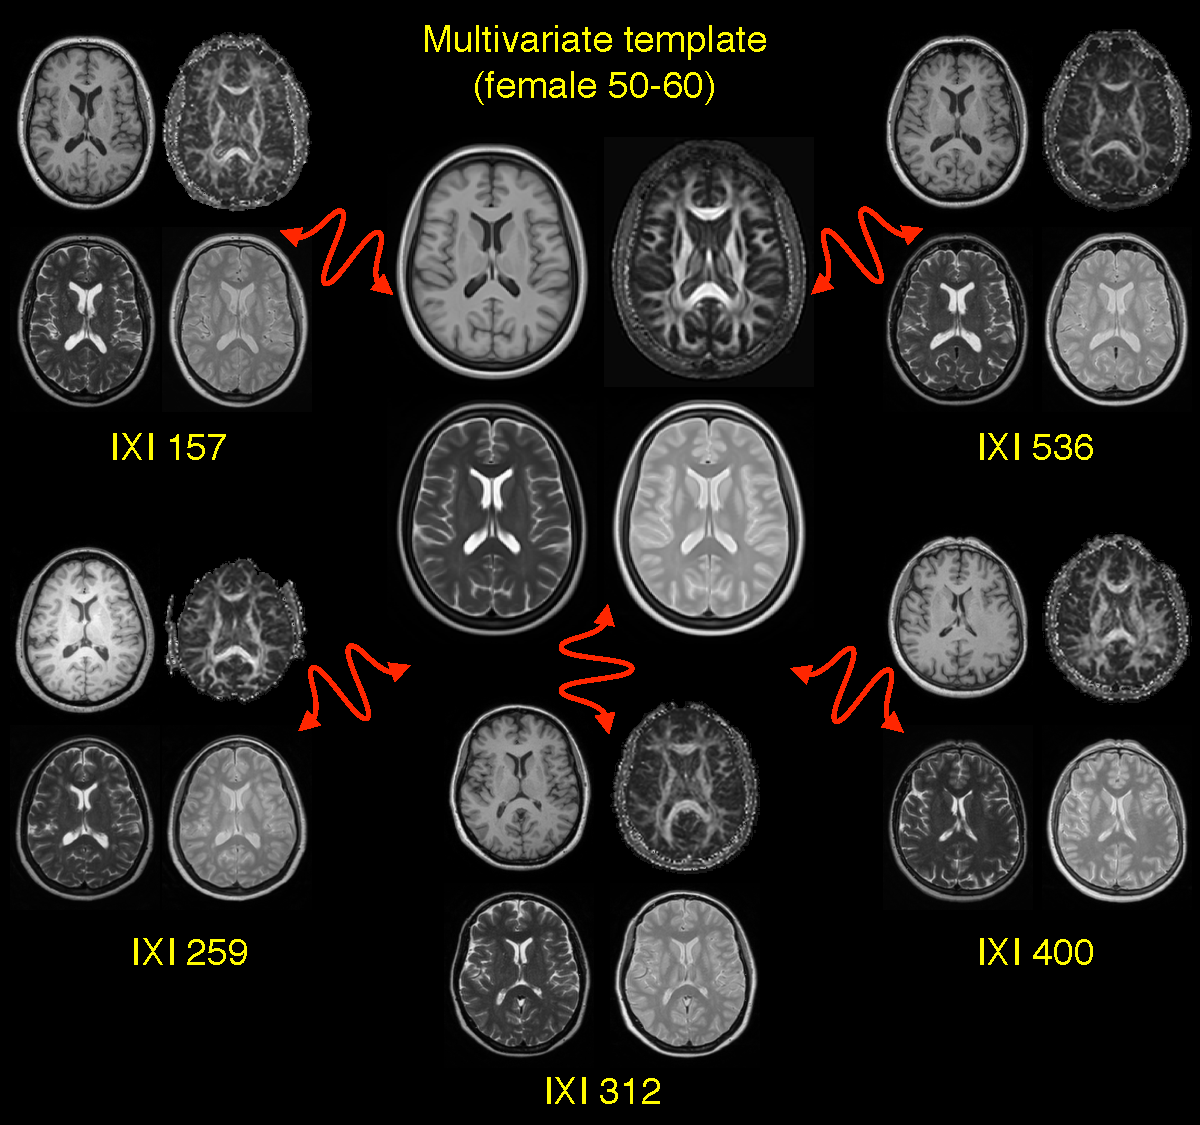
\includegraphics[width=90mm]{figs/template50_60.pdf}
  \caption{Sample multivariate template constructed from a subset of the IXI data (female, age 50--60).  Axial slices of five of the 37 total subjects from this cohort are shown. }
  \label{fig:template}
\end{figure}


